\documentclass{article}[11pt]
\usepackage{xparse}
\usepackage{fancyhdr}
\usepackage{pgf,tikz}
\usepackage[utf8]{inputenc}
\usepackage[T1]{fontenc}
\usepackage{listings}
\usepackage{xcolor}
\usepackage{graphicx}
\usepackage{amsmath}
\usepackage[a4paper,left=2cm,right=2cm,top=2.5cm,bottom=2cm]{geometry}
\usepackage{amsmath}
\usepackage{amssymb}
\usepackage{array}
\usepackage{pifont}
\usepackage{makecell}
\usepackage{xcolor}
\usepackage[]{algorithm2e}

% NEW COMMANDS & DEFINE
\definecolor{pythonColor}{HTML}{B634F6}
\definecolor{codegreen}{rgb}{0,0.6,0}
\definecolor{codegray}{rgb}{0.5,0.5,0.5}
\definecolor{codered}{rgb}{1.0,0.2,0.2}
\definecolor{codeyellow}{rgb}{1.0,1.0,0.2}
\definecolor{codepurple}{rgb}{0.58,0,0.82}
\definecolor{backcolour}{rgb}{1.0,1.0,1.0}
\lstdefinestyle{mystyle}{
    backgroundcolor=\color{backcolour},
    commentstyle=\color{codepurple},
    keywordstyle=\color{magenta},
    numberstyle=\tiny\color{codegray},
    stringstyle=\color{codepurple},
    basicstyle=\ttfamily\footnotesize,
    breakatwhitespace=true,
    breaklines=true,
    % captionpos=b,
    keepspaces=true,
    numbers=left,
    numbersep=10pt,
    showspaces=false,
    showstringspaces=false,
    showtabs=false,
    tabsize=2,
    frame=false
}

\lstset{style=mystyle}
\newcommand{\python}[1]{\textcolor{pythonColor}{\textit{#1}}}
\renewcommand{\headrulewidth}{0.5pt}
\renewcommand{\footrulewidth}{0.5pt}
\newcommand{\showCode}[1]{\lstinputlisting[language=Python]{#1}}


% DOCUMENTS SETTINGS
\newcommand{\titre}{Factorisations matricielles}
\newcommand{\devoir}{Analyse Numérique : Devoir 2}
\newcommand{\auteur}{Romain Graux}
\newcommand{\noma}{28681700}
\newcommand{\mytitle}{
    \raggedbottom
    \lhead{\auteur}
    \rhead{Novembre 2019}
    \lfoot{28681700}
    \rfoot{\titre}
    \pagestyle{fancy}
    \begin{center}
        \huge{{\textbf{\devoir}}}

        \Huge{\textit{\textbf{\titre}}}
    \end{center}
    \vspace{0.7cm}
}

\graphicspath{res/plots/}

\begin{document}
\mytitle
\section{LU}
\subsection{Factorisation}

Cette factorisation a pour but de factoriser la matrice initiale \python{A} en une matrice \textit{triangulaire inférieure} \python{L} et une matrice \textit{triangulaire supérieure} \python{U} ainsi, {A = LU}.
Cette factorisation cherche d'abord a faire un \textit{pivotage partiel}, ainsi les lignes sont échangées pour mettre les éléments maximums sous la diagonale sur l'élément de la diagonale, de cette manière on évitera par la suite de diviser par zéro lorsque l'on divisera par le pivot. Ensuite, on applique les \textit{éliminiations de Gauss} de manière itérative sur chaque éléments de \python{L} et de \python{U}. Comme nous sommes en Python, j'ai cherché à vectoriser un maximum de boucles, ce qui nous donne l'algorithme de 3 lignes suivant une fois la matrice pivotée:
\showCode{res/py/LU.py}

\subsection{Résolution}

Ayant \python{A} comme étant deux \textit{matrices triangulaires}, nous pouvons résoudre de la manière suivante en appliquant pour la résolution avec \python{L}, une substitution avant et avec \python{U}, une substitiution arrière.
\begin{align*}
    Ax&=b \\
    LUx&=b \\
    Ly&=b \\
    Ux&=y
\end{align*}

\section{Factorisation QR}

\section{Analyse}
\subsection{Complexité temporelle sur maillages différents}
\begin{figure}[!h]
    \centering
    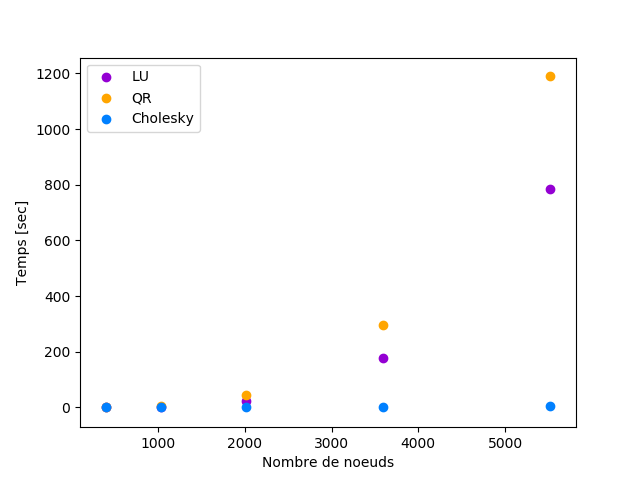
\includegraphics[width=18cm]{res/plots/complexite.png}
    \caption{Complexité temporelle de résolution avec LU et QR}
    \label{fig:compRef}
\end{figure}
\subsection{Complexité temporelle sur régimes différents}
\begin{figure}[!h]
    \centering
    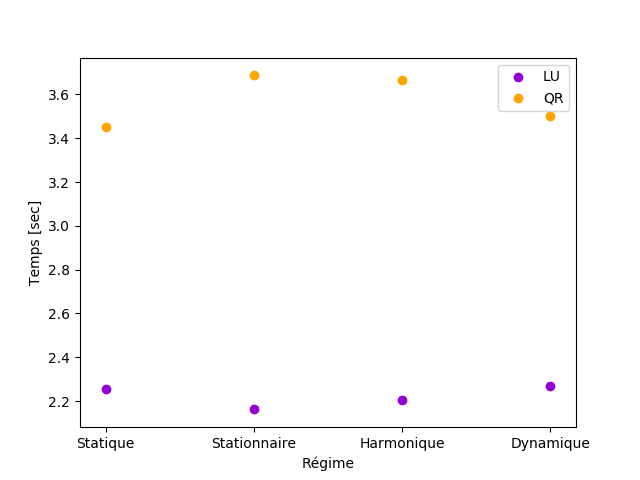
\includegraphics[width=18cm]{res/plots/regimes.png}
    \caption{Complexité temporelle de résolution avec LU et QR sur les 4 régimes}
    \label{fig:compReg}
\end{figure}

\end{document}
